% ------------------------------------------------------------------------
% ------------------------------------------------------------------------
% abnTeX2: Modelo de Trabalho Acadêmico (tese de doutorado, dissertação de
% mestrado e trabalhos monográficos em geral) em conformidade com 
% ABNT NBR 14724:2011: Informação e documentação - Trabalhos acadêmicos -
% Apresentação
% ------------------------------------------------------------------------
% ------------------------------------------------------------------------

\documentclass[12pt,openright,oneside,a4paper]{abntex2}	% frente e verso
%\documentclass[12pt,oneside,a4paper]{abntex2}			% apenas frente

% ---
% Pacotes fundamentais 
% ---
\usepackage{cmap}				% Mapear caracteres especiais no PDF
\usepackage{lmodern}			% Usa a fonte Latin Modern			
\usepackage[T1]{fontenc}		% Seleção de códigos de fonte.
\usepackage[utf8]{inputenc}		% Determina a codificação utiizada (conversão automática dos acentos)
\usepackage{makeidx}            % Cria o indice
\usepackage{hyperref}  			% Controla a formação do índice
\usepackage{lastpage}			% Usado pela Ficha catalográfica
\usepackage{indentfirst}		% Indenta o primeiro parágrafo de cada seção.
\usepackage{nomencl} 			% Lista de simbolos
\usepackage{color}				% Controle das cores
\usepackage{graphicx}			% Inclusão de gráficos
% ---
	
% ---
% Pacotes adicionais, usados apenas no âmbito do Modelo Canônico do abnteX2
% ---
\usepackage{lipsum}				% para geração de dummy text
% ---

% ---
% Pacotes de citações
% ---
\usepackage[brazilian,hyperpageref]{backref}	 % Paginas com as citações na bibl
\usepackage[alf]{abntex2cite}	% Citações padrão ABNT
% --- 
% CONFIGURAÇÕES DE PACOTES
% --- 
\graphicspath{{imagens/}} 
% ---
% Configurações do pacote backref
% Usado sem a opção hyperpageref de backref
\renewcommand{\backrefpagesname}{Citado na(s) página(s):~}
% Texto padrão antes do número das páginas
\renewcommand{\backref}{}
% Define os textos da citação
\renewcommand*{\backrefalt}[4]{
	\ifcase #1 %
		Nenhuma citação no texto.%
	\or
		Citado na página #2.%
	\else
		Citado #1 vezes nas páginas #2.%
	\fi}%
% ---

% ---
% Informações de dados para CAPA e FOLHA DE ROSTO
% ---
\titulo{SEARCHLIGHT: Facilitando a visualização de informações crowdsourcing em Mapas Web atravéss de Zoom}
\autor{Wancharle Sebastião Quirino}
\local{Vitória - ES, Brasil}
\data{XX de maio de 2013}
\orientador{Celso Alberto Saibel Santos}
\instituicao{%
  Universidade Federal do Espírito Santo
  \par
  Centro Tecnológico
  \par
  Departamento de Informática}
\tipotrabalho{Trabalho de Conclusão de Curso}
% O preambulo deve conter o tipo do trabalho, o objetivo, 
% o nome da instituição e a área de concentração 
\preambulo{Monografia apresentada para obtenção do Grau de Bacharel em Engenharia de Computação pela Universidade Federal do Espírito Santo.}
% ---





% ---
% Configurações de aparência do PDF final

% alterando o aspecto da cor azul
\definecolor{blue}{RGB}{41,5,195}

% informações do PDF
\hypersetup{
     	%backref=true,
     	%pagebackref=true,
		%bookmarks=true,         		% show bookmarks bar?
		pdftitle={\imprimirtitulo}, 
		pdfauthor={\imprimirautor},
    	pdfsubject={\imprimirpreambulo},
		pdfkeywords={PALAVRAS}{CHAVES}{abnt}{abntex}{abntex2},
	    pdfproducer={LaTeX with abnTeX2}, 	% producer of the document
	    pdfcreator={\imprimirautor},
    	colorlinks=true,       		% false: boxed links; true: colored links
    	linkcolor=blue,          	% color of internal links
    	citecolor=blue,        		% color of links to bibliography
    	filecolor=magenta,      		% color of file links
		urlcolor=blue,
		bookmarksdepth=4
}
% --- 

% --- 
% Espaçamentos entre linhas e parágrafos 
% --- 

% O tamanho do parágrafo é dado por:
\setlength{\parindent}{1.3cm}

% Controle do espaçamento entre um parágrafo e outro:
\setlength{\parskip}{0.2cm}  % tente também \onelineskip

% Controles do espaçamento entre linhas:
%\OnehalfSpacing	% espaçamento um e meio (padrão); 
%\DoubleSpacing		% espaçamento duplo
%\SingleSpacing		% espaçamento simples	
% --- 
	

% ---
% compila o indice
% ---
\makeindex
% ---
\makenomenclature
% ---

% ----
% Início do documento
% ----
\begin{document}

% ----------------------------------------------------------
% ELEMENTOS PRÉ-TEXTUAIS
% ----------------------------------------------------------
% \pretextual

% ---
% Capa
% ---
\imprimircapa
% ---

% ---
% Folha de rosto
% (o * indica que haverá a ficha bibliográfica)
% ---
\imprimirfolhaderosto*
% ---

% ---
% Inserir a ficha bibliografica
% ---

% Isto é um exemplo de Ficha Catalográfica, ou ``Dados internacionais de
% catalogação-na-publicação''. Você pode utilizar este modelo como referência. 
% Porém, provavelmente a biblioteca da sua universidade lhe fornecerá um PDF
% com a ficha catalográfica definitiva após a defesa do trabalho. Quando estiver
% com o documento, salve-o como PDF no diretório do seu projeto e substitua todo
% o conteúdo de implementação deste arquivo pelo comando abaixo:
%
% \begin{fichacatalografica}
%     \includepdf{fig_ficha_catalografica.pdf}
% \end{fichacatalografica}
% ---


% ---
% Inserir folha de aprovação
% ---

% Isto é um exemplo de Folha de aprovação, elemento obrigatório da NBR
% 14724/2011 (seção 4.2.1.3). Você pode utilizar este modelo até a aprovação
% do trabalho. Após isso, substitua todo o conteúdo deste arquivo por uma
% imagem da página assinada pela banca com o comando abaixo:
%
% \includepdf{folhadeaprovacao_final.pdf}
%
\begin{folhadeaprovacao}

  \begin{center}
    \vspace*{1cm}
    {\ABNTEXchapterfont\large\imprimirautor}

    \vspace*{\fill}\vspace*{\fill}
    {\ABNTEXchapterfont\bfseries\Large\imprimirtitulo}
    \vspace*{\fill}
    
    \hspace{.45\textwidth}
    \begin{minipage}{.5\textwidth}
        \imprimirpreambulo
    \end{minipage}%
    \vspace*{\fill}
   \end{center}
    
   Trabalho aprovado. \imprimirlocal, 24 de novembro de 2012:

   \assinatura{\textbf{\imprimirorientador} \\ Orientador} 
   \assinatura{\textbf{Professor} \\ Convidado 1}
   \assinatura{\textbf{Professor} \\ Convidado 2}
   %\assinatura{\textbf{Professor} \\ Convidado 3}
   %\assinatura{\textbf{Professor} \\ Convidado 4}
      
   \begin{center}
    \vspace*{0.5cm}
    {\large\imprimirlocal}
    \par
    {\large\imprimirdata}
    \vspace*{1cm}
  \end{center}
  
\end{folhadeaprovacao}
% ---

% ---
% Dedicatória
% ---
\begin{dedicatoria}
   \vspace*{\fill}
   \noindent
   \begin{flushright}
   
   \textit{ Este trabalho é dedicado aos meus pais,  que sempre estiveram comigo, \\ por toda a sua dedicação.}
   \end{flushright}
   
\end{dedicatoria}
% ---

% ---
% Agradecimentos
% ---
\begin{agradecimentos}
Os agradecimentos principais são direcionados a  ...

Agradecimentos especiais são direcionados a ...

\end{agradecimentos}
% ---

% ---
% Epígrafe
% ---

% ---

% ---
% RESUMOS
% ---

% resumo em português
\begin{resumo}
 Segundo a citeonline[3.1-3.2]{NBR6028:2003}, o resumo deve ressaltar o
 objetivo, o método, os resultados e as conclusões do documento. A ordem e a extensão
 destes itens dependem do tipo de resumo (informativo ou indicativo) e do
 tratamento que cada item recebe no documento original. O resumo deve ser
 precedido da referência do documento, com exceção do resumo inserido no
 próprio documento. (\ldots) As palavras-chave devem figurar logo abaixo do
 resumo, antecedidas da expressão Palavras-chave:, separadas entre si por
 ponto e finalizadas também por ponto.

 \vspace{\onelineskip}
    
 \noindent
 \textbf{Palavras-chaves}: latex. abntex. editoração de texto.
\end{resumo}

% resumo em inglês
\begin{resumo}[Abstract]
 This is the english abstract.

 \vspace{\onelineskip}
 
 \noindent 
 \textbf{Key-words}: latex. abntex. text editoration.
\end{resumo}

% ---

% ---
% inserir lista de ilustrações
% ---
\pdfbookmark[0]{\listfigurename}{lof}
\listoffigures*
\cleardoublepage
% ---

% ---
% inserir lista de tabelas
% ---
\pdfbookmark[0]{\listtablename}{lot}
\listoftables*
\cleardoublepage
% ---

% ---
% inserir lista de abreviaturas e siglas
% A lista de Abreviaturas e Siglas pode ser facilmente montada com o pacote 
% nomencl. Abaixo segue um exemplo.
% ---
\nomenclature{Fig.}{Figura}
\nomenclature{$A_i$}{Area of the $i^{th}$ component} 
\nomenclature{456}{Isto é um número}
\nomenclature{123}{Isto é outro número}
\nomenclature{a}{primeira letra do alfabeto}
\nomenclature{lauro}{este é meu nome} 

\renewcommand{\nomname}{Lista de abreviaturas e siglas}
\pdfbookmark[0]{\nomname}{las}
\printnomenclature
\cleardoublepage
% ---

% ---
% inserir lista de símbolos
% ---
% O abnTeX2 não provê mecanismo para lista de símbolos.
% ---

% ---
% inserir o sumario
% ---
\pdfbookmark[0]{\contentsname}{toc}
\tableofcontents*
\cleardoublepage
% ---



% ----------------------------------------------------------
% ELEMENTOS TEXTUAIS
% ----------------------------------------------------------
% É possível usar \textual ou \mainmatter, que é a macro padrão do memoir.  
\mainmatter

% ----------------------------------------------------------
% Introdução
% ----------------------------------------------------------
\chapter[Introdução]{Introdução}

\section{Contextualização}
O estado atual da comunicação mundial permite as pessoas, de qualquer país, comunicar e trocar conhecimento dos mais diversos assuntos. Essa facilidade de comunicação também facilita a união de indivíduos, que não se conhecem e com realidades sociais completamente opostas, em um projeto com metas em comum.

Um exemplo, dessa união incomum, é o caso de um carpinteiro sul-africano que, ao perder os dedos numa serra, e ficar insatisfeito com os preços e qualidade das próteses disponíveis no mercado, resolveu iniciar um projeto open source de mão biônica com a ajuda de um técnico de efeitos especiais que mora nos EUA. Juntos, esses dois indíviduos que até então não se conheciam, conseguiram criar um projeto de mão biônica por 150 dólares. Após isso, o projeto ganhou visibilidade e patrocínio e já está sendo testado por algumas crianças deficientes da africa do sul\footnote{\label{maobionica} Notícia sobre projeto de mão biônica \url{http://meiobit.com/115807/}}.

Essa melhoria de comunicação, obviamente, também  afeta o campo empresarial. Em algumas empresas, o sistema de "Outsourcing", que é um sistema de aquisição de conhecimento ou tecnologia, começou a ser substituído pelo sistema de "Crowndsourcing", que no campo empresarial, funciona como uma espécie de concorrência: a empresa lança uma espécie de edital informando quanto pode pagar por determinada solução e quem quer que seja poderá oferecer a resposta adequada ao que se procura, independente de ser uma, duas, ou cem pessoas, contanto que resolva o problema.

De modo geral Crowdsourcing é a prática de obtenção de serviços, idéias ou conteúdo solicitando contribuições de um grande grupo de pessoas e, especialmente, a partir de uma comunidade on-line, ao invés de funcionários ou fornecedores tradicionais \footnote{\label{wiki-crowd} Definição completa de crowdsourcing \url{ http://en.wikipedia.org/wiki/Crowdsourcing}}.
Existem diversos tipos de crowdsourcing, mas nesse trabalho iremos nos focar no crowdsourcing conhecido como \emph{Wisdom of the Crowd} que é um tipo de crowdsourcing que coleta grandes quantidades de informação e as agrega para obter uma visão completa e precisa sobre um determinado tema. Essa visão, dependendo do tema de estudo, pode ser representada por um mapa de crowdsourcing.

A produção de mapas crowdsourcing é geralmente feita de forma automática, usualmente temos algum software e/ou site que coleta as informações e as agrupa por meio de algum algorítimo desenvolvido especificamente para o mapa.

A coleta dessas informações pode ocorrer de várias formas, tanto manual como automática. Por exemplo, no site \citeauthoronline{portoalegre} os usuários podem adicionar novas informações através do site, ou seja, ela é feita de forma manual. Alguns sistemas podem coletar informações de forma automática usando programas de computadores, aplicativos de smartphones \cite{thiagarajan_cooperative_2010}  e até mesmo da internet\footnote{ Mapa com informações coletadas do Twitter \url{http://trendsmap.com}}.

Uma vez coletada, essa informação é analisada e exibida em um mapa, mas o mapa em si não é o produto final, e sim algumas informações específicas retiradas dele. Por exemplo, podemos ter mapas que mostrem os congestionamentos no trânsito de uma cidade e um sistema \cite{thiagarajan_vtrack:_2009} que através desse mapa consegue identificar  uma rota mais eficiente com menor consumo de energia, evitando assim ficar parado no congestionamento gastando gasolina.

Em alguns casos, mapas de crowdsourcing possuem informações posicionadas em regiões muito próximas entre si, que devido a quantidade elevada, acabam poluindo a visualização e dificultando a compreensão do mapa. Esse problema pode ser resolvido quando os mapas oferecem mecanismos para agrupar e filtrar essas informações. Um mecanismo ideal é o zoom contextual ou zoom em grupo, que filtra informações irrelevantes, em determinados níveis de zoom, deixando o mapa mais leve e compreensível.

O Projeto Searchlight pretende ser uma ferramenta para auxiliar e melhorar a visualização de mapas de crowdsourcing.

O escopo do projeto atinge a criação de uma ferramenta que visualize mapas de crowdsourcing em um navegador de internet, tanto desktop quanto mobile, usando recursos de visualização de mapas já disponíveis em HTML5 mas que ainda não possuem zoom contextual e outras opções úteis que permitam uma melhor visualização do mapa.



\section{Definição do Problema}
Mapas de crowdsourcing tendem a mostrar uma enorme quantidade de informação. Essa característica faz com que, em alguns casos, a visualização e a compreensão do mapa seja comprometida.
 
Ao trabalhar com mapas de crowdsourcing, geralmente encontramos 2 problemas: a sobreposição de informações e o zoom arbitrário. 



\subsection{Sobreposição de Informações}
O site \citeauthoronline{portoalegre} é um exemplo da importância do mapas de crowdsourcing no contexto governamental e na sociedade. Por meio desse site os cidadãos de porto alegre podem relatar os problemas de sua cidade para que as autoridades tomem as devidas providências. 

Um dos principais objetivos do site é identificar as áreas prioritárias em que o governo deveria atuar. Mas a sobreposição de informações dificulta essa tarefa, pois ocorre frequentemente nesse site. 

\begin{figure}[htb]
	\caption{\label{fig-porto-alegre} Sobreposição de informações no mapa do site PortoAlegre.cc}
	\begin{center}
	    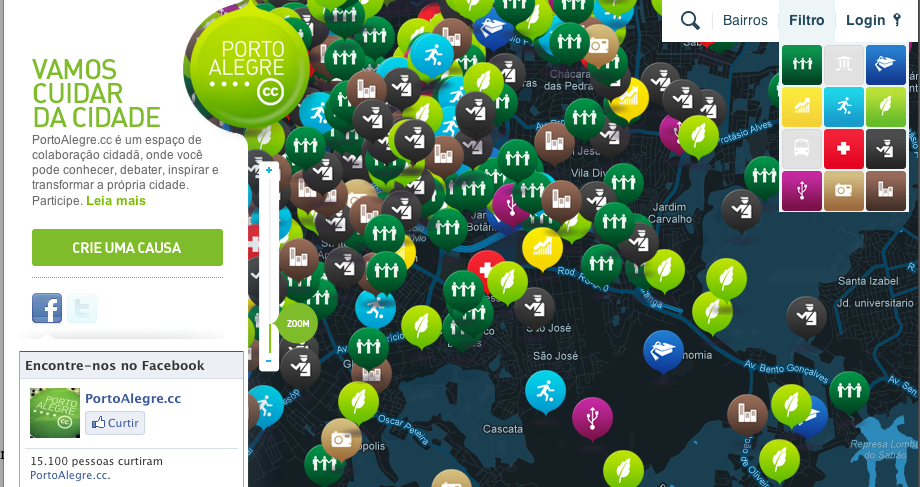
\includegraphics[scale=0.4]{portoalegre-cc}
	\end{center}
	\legend{Fonte: \citeonline{portoalegre}}
\end{figure}

Esse problema fica evidente na \autoref{fig-porto-alegre} quando consideramos, a possibilidade, que um grupo de 5 marcadores reunidos numa região específica, podem sobrepor dezenas ou até milhares de outros marcadores. Ou seja, o mapa não consegue mostrar, com clareza e precisão, as áreas de maior ocorrência de determinado incidente. 

O site fornece um filtro por categorias, que diminui de forma significativa a quantidade de informação exibida.  Mas infelizmente não resolve o problema, pois a sobreposição de informação ainda pode ocorrer com informações de uma mesma categoria.





\subsection{Zoom arbitrário}
Alguns sites criam mecanismos que minimizam o problema da sobreposição de informações. Como exemplo, temos o \citeonline{crimemapatl}  mostrado na \autoref{fig-mapatl} que mostra um mapa com a taxa de crimes em Atlanta. 

O site fornece filtros por categoria, data e zoom. Mas o principal responsável pela eliminação da sobreposição de informação é o filtro por zoom. Esse filtro agrupa todos os marcadores que estão sobrepostos, no zoom atual, em um único marcador que exibe a informação somada dos marcadores que o compõem.
 
\begin{figure}[htb]
	\caption{\label{fig-mapatl} MapATL não possui sobreposição de informação devido ao filtro por zoom}
	\begin{center}
	    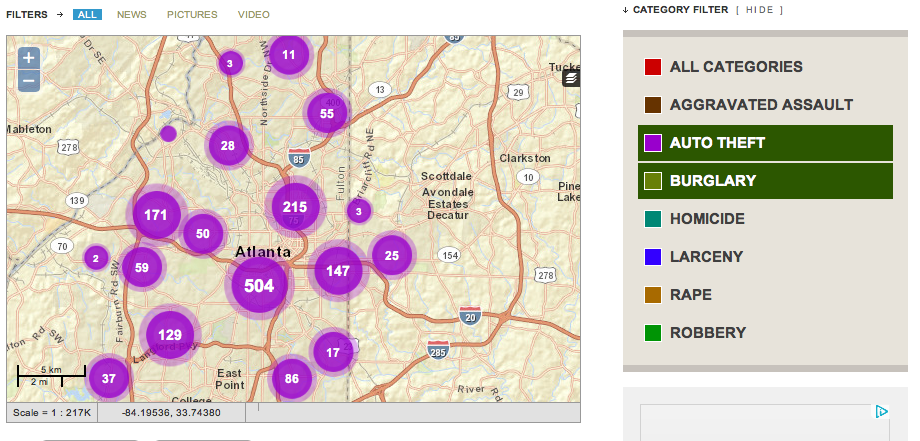
\includegraphics[scale=0.4]{crime-mapatl-com-filtro}
	\end{center}
	\legend{Fonte: \citeonline{crimemapatl}}
\end{figure}

Segundo \cite[42,44]{silva2010solap+} esse tipo de agrupamento, baseado em grelha, pode ser implementado a partir do algorítimo WaveCluster\cite{wavecluster}. 

 

\begin{figure}[htb]
	\caption{\label{fig-zoomab} Entre ZOOM A e ZOOM C existem muitos níveis intermediários e não apenas 1 (ZOOM B).}
	\begin{center}
	    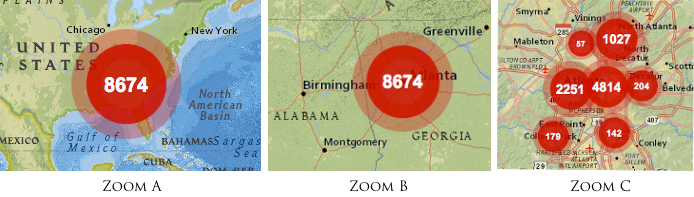
\includegraphics[scale=0.6]{zoomab}
	\end{center}
	\legend{Fonte: \citeonline{crimemapatl}}
\end{figure}

Esse algorítimo resolve o problema de sobreposição de informações. Porém o problema do zoom arbitrário, ilustrado na \autoref{fig-zoomab}, permanece.

O usuário precisa aplicar vários zoons para ir do ZOOM A para o ZOOM C. Mas durante essa interação é gasto tempo e banda, da conexão de internet, do usuário para exibir os zoons intermediários, quando o ideal seria exibir apenas o ZOOM B.

Esse gasto de banda, prejudica a usabilidade de mapas em dispositivos móveis pois, geralmente, eles possuem pouca banda de internet.

Uma abordagem para esse problema é o uso de um zoom inteligente que siga uma hierarquia espacial invés de simplesmente dobrar a visualização atual. 

\subsubsection{Informações arbitrárias}
Um subproblema do zoom arbitrário é a exibição de informações desnecessárias em todos os níveis de zoom. Na \autoref{fig-mapaufes} podemos observar o problema, que neste caso, a arbitrariedade está na exibição de informações, e não no número de zoons. 
 \begin{figure}[htb]
	\caption{\label{fig-mapaufes}Informações necessárias em níveis superiores, de zoom, visualizadas em níveis inferiores}
	\begin{center}
	    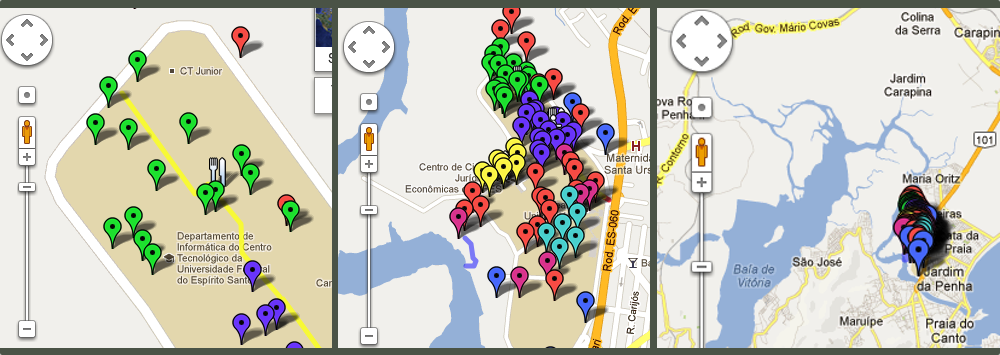
\includegraphics[scale=0.4]{ufes_map}
	\end{center}
	\legend{Fonte: http://maps.google.com}
\end{figure}
Os marcadores desse mapa exibem informações sobre os departamentos internos da UFES, mas essas informações são úteis apenas em certos níveis de zoom. Em níveis mais baixos, onde a área dessa universidade seja desprezível, a informação perde seu valor e fica poluindo o mapa. Neste caso, um único marcador representando o grupo seria mais útil.

\section{Objetivos}
Com base nas informações da definição do problema, o objetivo deste trabalho é desenvolver uma ferramenta que: agrupe marcadores de forma inteligente eliminando a sobreposição; forneça um zoom inteligente que não exiba níveis intermediários desnecessários; esconda marcadores quando sua informação não seja mais necessária ao nível observado.

O objetivo principal desse trabalho é facilitar a visualização de informação em mapas crowdsourcing. Isso devido a importância sócio-econômica das informações que geralmente são exibidas nessa classe de mapas. Mas a ferramenta poderia implementar recursos que também facilite a divulgação dessas informações. Por isso, o objetivo secundário é fornecer um mecanismo para gerar mapas a partir de planilhas de dados, e compartilhá-los sem que o autor precise programar ou ter algum conhecimento de programação. Para este trabalho a divulgação dos mapas é um objetivo secundário, mas poderia ser melhor abordado em trabalhos futuros.
  
\section{Contribuições}
A contribuição deste trabalho é o desenvolvimento de um framework para exibição de mapas em paginas web facilitando a visualização de informações crowdsourcing.

Além disso também foi criado um website do projeto\cite{gitsite} que explica e documenta o framework. O website fornece também um pagina de geração e compartilhamento de mapas por pessoas que não sabem programar.

\section{Estrutura da Monografia}
Este trabalho está organizado da seguinte forma:

Nesta introdução, é apresentado o contexto geral do projeto, a definição do problema, a solução proposta e a estrutura da monografia.

No capítulo 2, Fundamentação Teórica, apresenta-se uma explicação básica sobre os elementos comuns em mapas geográficos, usados na web, e suas relações com crowdsourcing; uma pesquisa sobre as estratégias para lidar com mapas que possuem muitos marcadores; uma pesquisa sobre algorítimos para agrupamento de pontos; uma revisão sobre o uso de planilhas eletrônicas como principal ambiente de programação para usuários finais em órgãos governamentais e seus usos como base de dados para informações geográficas.

No capítulo 3, Desenvolvimento, é explicado como o projeto foi desenvolvido, quais foram as ferramentas utilizadas, e o motivo da escolha de determinadas tecnologias. 

No capítulo 4, Solução Desenvolvida, é apresentado em detalhes a solução que foi desenvolvida e como utilizá-la.

No capitulo 5, Conclusão, é apresentado as dificuldades encontradas no decorrer do projeto, trabalhos futuros e conclusão geral sobre o projeto.






% ----------------------------------------------------------
% PARTE - preparação da pesquisa
% ----------------------------------------------------------
\chapter{Pesquisa}





% ----------------------------------------------------------
% Parte de revisãod e literatura
% ----------------------------------------------------------
\chapter{Desenvolvimento}
\section{Arquitetura do Framework}
\section{Ferramentas Utilizadas no Desenvolvimento}
\subsection{Leaftetjs}
\subsection{GeoDjango}


% ---
% Capitulo de revisão de literatura
% ---


% ----------------------------------------------------------
% Resultados
% ----------------------------------------------------------
\chapter{Resultados}
% ----------------------------------------------------------
% Capitulo com exemplos de comandos inseridos de arquivo externo 
% ----------------------------------------------------------

%%% abtex2-modelo-include-comandos.tex, v-1.4 laurocesar
%% Copyright 2012-2013 by abnTeX2 group at http://abntex2.googlecode.com/ 
%%
%% This work may be distributed and/or modified under the
%% conditions of the LaTeX Project Public License, either version 1.3
%% of this license or (at your option) any later version.
%% The latest version of this license is in
%%   http://www.latex-project.org/lppl.txt
%% and version 1.3 or later is part of all distributions of LaTeX
%% version 2005/12/01 or later.
%%
%% This work has the LPPL maintenance status `maintained'.
%% 
%% The Current Maintainer of this work is the abnTeX2 team, led
%% by Lauro César Araujo. Further information are available on 
%% http://abntex2.googlecode.com/
%%
%% This work consists of the files abntex2-modelo-include-comandos.tex
%%

% ---
% Este capítulo, utilizado por diferentes exemplos do abnTeX2, ilustra o uso de
% comandos do abnTeX2 e de LaTeX.
% ---
 
\chapter{Resultados de comandos}\label{cap_exemplos}

\chapterprecis{Isto é uma sinopse de capítulo. A ABNT não traz nenhuma
normatização a respeito desse tipo de resumo, que é mais comum em romances 
e livros técnicos.}\index{sinopse de capítulo}

% ---
\section{Codificação dos arquivos: UTF8}
% ---

A codificação de todos os arquivos do \abnTeX2 é \texttt{UTF8}. É necessário que
você utilize a mesma codificação nos documentos que escrever, inclusive nos
arquivos de base bibliográficas |.bib|.

% ---
\section{Citações}
% ---

\index{citações!diretas}Utilize o ambiente \texttt{citacao} para incluir
citações diretas com mais de três linhas:

\begin{citacao}
As citações diretas, no texto, com mais de três linhas, devem ser
destacadas com recuo de 4 cm da margem esquerda, com letra menor que a do texto
utilizado e sem as aspas. No caso de documentos datilografados, deve-se
observar apenas o recuo \cite[5.3]{NBR10520:2002}
\end{citacao}

\index{citações!simples}Citações simples, com até três linhas, devem ser
incluídas com aspas. Observe que em \LaTeX as aspas iniciais são diferentes das finais: ``Amor é fogo que
arde sem se ver''.


% ---
\section{Remissões internas}
% ---

Ao nomear a \autoref{tab-nivinv}, apresentamos um exemplo de remissão interna,
que também pode ser feita quando indicamos o \autoref{cap_exemplos}\footnote{O
número do capítulo indicado é
\ref{cap_exemplos}, que se inicia à página \pageref{cap_exemplos}.}
(\nameref{cap_exemplos}, \autopageref{cap_exemplos}), por exemplo.

% ---
\section{Tabelas}
% ---

\index{tabelas}A \autoref{tab-nivinv} é um exemplo de tabela construída em
\LaTeX.

\begin{table}[htb]
\footnotesize
\caption[Níveis de investigação]{Níveis de investigação.}
\label{tab-nivinv}
\begin{tabular}{p{2.6cm}|p{6.0cm}|p{2.25cm}|p{3.40cm}}
  %\hline
   \textbf{Nível de Investigação} & \textbf{Insumos}  & \textbf{Sistemas de Investigação}  & \textbf{Produtos}  \\
    \hline
    Meta-nível & Filosofia\index{filosofia} da Ciência  & Epistemologia &
    Paradigma  \\
    \hline
    Nível do objeto & Paradigmas do metanível e evidências do nível inferior &
    Ciência  & Teorias e modelos \\
    \hline
    Nível inferior & Modelos e métodos do nível do objeto e problemas do nível inferior & Prática & Solução de problemas  \\
   % \hline
\end{tabular}
\legend{Fonte: \citeonline{van86}}
\end{table}

% ---
\section{Expressões matemáticas}
% ---

\index{expressões matemáticas}Use o ambiente \texttt{equation} para escrever
expressões matemáticas numeradas:

\begin{equation}
  \forall x \in X, \quad \exists \: y \leq \epsilon
\end{equation}

Escreva expressões matemáticas entre \$ e \$, como em $ \lim_{x \to \infty}
\exp(-x) = 0 $, para que fiquem na mesma linha.

Também é possível usar colchetes para indicar o início de uma expressão
matemática que não é numerada.

\[
\left|\sum_{i=1}^n a_ib_i\right|
\le
\left(\sum_{i=1}^n a_i^2\right)^{1/2}
\left(\sum_{i=1}^n b_i^2\right)^{1/2}
\]

Consulte mais informações sobre expressões matemáticas em
\url{http://code.google.com/p/abntex2/w/edit/Referencias}.

\section{Figuras}

\index{figuras}Figuras podem ser criadas diretamente em \LaTeX,
como o exemplo da \autoref{fig_circulo}.

\begin{figure}[htb]
	\caption{\label{fig_circulo}A delimitação do espaço}
	\begin{center}
	    \setlength{\unitlength}{5cm}
		\begin{picture}(1,1)
		\put(0,0){\line(0,1){1}}
		\put(0,0){\line(1,0){1}}
		\put(0,0){\line(1,1){1}}
		\put(0,0){\line(1,2){.5}}
		\put(0,0){\line(1,3){.3333}}
		\put(0,0){\line(1,4){.25}}
		\put(0,0){\line(1,5){.2}}
		\put(0,0){\line(1,6){.1667}}
		\put(0,0){\line(2,1){1}}
		\put(0,0){\line(2,3){.6667}}
		\put(0,0){\line(2,5){.4}}
		\put(0,0){\line(3,1){1}}
		\put(0,0){\line(3,2){1}}
		\put(0,0){\line(3,4){.75}}
		\put(0,0){\line(3,5){.6}}
		\put(0,0){\line(4,1){1}}
		\put(0,0){\line(4,3){1}}
		\put(0,0){\line(4,5){.8}}
		\put(0,0){\line(5,1){1}}
		\put(0,0){\line(5,2){1}}
		\put(0,0){\line(5,3){1}}
		\put(0,0){\line(5,4){1}}
		\put(0,0){\line(5,6){.8333}}
		\put(0,0){\line(6,1){1}}
		\put(0,0){\line(6,5){1}}
		\end{picture}
	\end{center}
	\legend{Fonte: os autores}
\end{figure}

Ou então figuras podem ser incorporadas de arquivos externos, como é o caso da
\autoref{fig_grafico}. Se a figura que ser incluída se tratar de um diagrama, um
gráfico ou uma ilustração que você mesmo produza, priorize o uso de imagens
vetoriais no formato PDF. Com isso, o tamanho do arquivo final do trabalho será
menor, e as imagens terão uma apresentação melhor, principalmente quando
impressas, uma vez que imagens vetorias são perfeitamente escaláveis para
qualquer dimensão. Nesse caso, se for utilizar o Microsoft Excel para produzir
gráficos, ou o Microsoft Word para produzir ilustrações, exporte-os como PDF e
os incorpore ao documento conforme o exemplo abaixo. No entanto, para manter a
coerência no uso de software livre (já que você está usando \LaTeX e \abnTeX),
teste a ferramenta \textsf{InkScape}\index{InkScape}
(\url{http://inkscape.org/}). Ela é uma excelente opção de código-livre para
produzir ilustrações vetoriais, similar ao CorelDraw\index{CorelDraw} ou ao Adobe
Illustrator\index{Adobe Illustrator}. De todo modo, caso não seja possível
utilizar arquivos de imagens como PDF, utilize qualquer outro formato, como
JPEG, GIF, BMP, etc. Nesse caso, você pode tentar aprimorar as imagens
incorporadas com o software livre \textsf{Gimp}\index{Gimp}
(\url{http://www.gimp.org/}). Ele é uma alternativa livre ao Adobe
Photoshop\index{Adobe Photoshop}.

\begin{figure}[htb]
	\caption{\label{fig_grafico}Gráfico produzido em Excel e salvo como PDF}
	\begin{center}
	    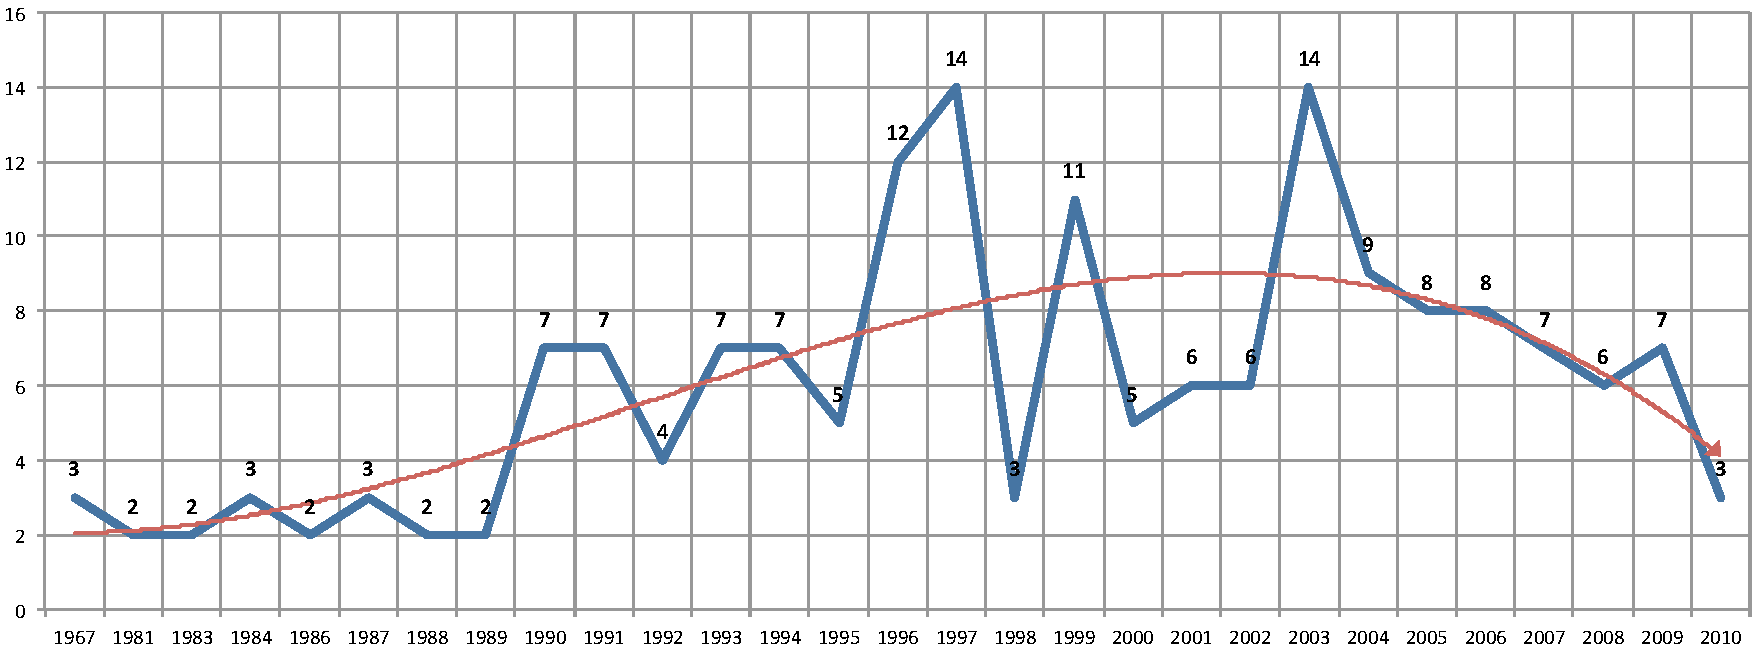
\includegraphics[scale=0.5]{abntex2-modelo-img-grafico.pdf}
	\end{center}
	\legend{Fonte: \citeonline[p. 24]{araujo2012}}
\end{figure}

% ---
\section{Enumerações: alíneas e subalíneas}
% ---

\index{alíneas}\index{subalíneas}\index{incisos}Quando for necessário enumerar
os diversos assuntos de uma seção que não possua título, esta deve ser
subdividida em alíneas \cite[4.2]{NBR6024:2012}:

\begin{alineas}

  \item os diversos assuntos que não possuam título próprio, dentro de uma mesma
  seção, devem ser subdivididos em alíneas\footnote{As notas devem ser digitadas ou datilografadas
  dentro das margens, ficando separadas do texto por um espaço simples de entre as
  linhas e por filete de 5 cm, a partir da margem esquerda. Devem ser
  alinhadas, a partir da segunda linha da mesma nota, abaixo da primeira letra
  da primeira palavra, de forma a destacar o expoente, sem espaço entre elas e
  com fonte menor. \citeonline[5.2.1]{NBR14724:2011}}; 
  
  \item o texto que antecede as alíneas termina em dois pontos;
  \item as alíneas devem ser indicadas alfabeticamente, em letra minúscula,
  seguida de parêntese. Utilizam-se letras dobradas, quando esgotadas as
  letras do alfabeto;

  \item as letras indicativas das alíneas devem apresentar recuo em relação à
  margem esquerda;

  \item o texto da alínea deve começar por letra minúscula e terminar em
  ponto-e-vírgula, exceto a última alínea que termina em ponto final;

  \item o texto da alínea deve terminar em dois pontos, se houver subalínea;

  \item a segunda e as seguintes linhas do texto da alínea começa sob a
  primeira letra do texto da própria alínea;
  
  \item subalíneas \cite[4.3]{NBR6024:2012} devem ser conforme as alíneas a
  seguir:

  \begin{alineas}
     \item as subalíneas devem começar por travessão seguido de espaço;

     \item as subalíneas devem apresentar recuo em relação à alínea;

     \item o texto da subalínea deve começar por letra minúscula e terminar em
     ponto-e-vírgula. A última subalínea deve terminar em ponto final, se não
     houver alínea subsequente;

     \item a segunda e as seguintes linhas do texto da subalínea começam sob a
     primeira letra do texto da própria subalínea.
  \end{alineas}
  
  \item no \abnTeX\ estão disponíveis os ambientes \texttt{incisos} e
  \texttt{subalineas}, que em suma são o mesmo que se criar outro nível de
  \texttt{alineas}, como nos exemplos à seguir:
  
  \begin{incisos}
    \item \textit{Um novo inciso em itálico};
  \end{incisos}
  
  \item Alínea em \textbf{negrito}:
  
  \begin{subalineas}
    \item \textit{Uma subalínea em itálico};
    \item \underline{\textit{Uma subalínea em itálico e sublinhado}}; 
  \end{subalineas}
  
  \item Última alínea com \emph{ênfase}.
  
\end{alineas}


% ---
\section{Espaçamento entre parágrafos e linhas}
% ---

\index{espaçamento!dos parágrafos}O tamanho do parágrafo, espaço entre a margem
e o início da frase do parágrafo, é definido por:

\begin{verbatim}
   \setlength{\parindent}{1.3cm}
\end{verbatim}

\index{espaçamento!do primeiro parágrafo}Por padrão, não há espaçamento no
primeiro parágrafo de cada início de divisão do documento
(\autoref{sec-divisoes}). Porém, você pode definir que o primeiro parágrafo
também seja indentado, como é o caso deste documento. Para isso, apenas inclua o
pacote \textsf{indentfirst} no preâmbulo do documento:

\begin{verbatim}
   \usepackage{indentfirst}      % Indenta o primeiro parágrafo de cada seção.
\end{verbatim}

\index{espaçamento!entre os parágrafos}O espaçamento entre um parágrafo e outro
pode ser controlado por meio do comando:

\begin{verbatim}
  \setlength{\parskip}{0.2cm}  % tente também \onelineskip
\end{verbatim}

\index{espaçamento!entre as linhas}O controle do espaçamento entre linhas é
definido por:

\begin{verbatim}
  \OnehalfSpacing       % espaçamento um e meio (padrão); 
  \DoubleSpacing        % espaçamento duplo
  \SingleSpacing        % espaçamento simples	
\end{verbatim}

Para isso, também estão disponíveis os ambientes:

\begin{verbatim}
  \begin{SingleSpace} ...\end{SingleSpace}
  \begin{Spacing}{hfactori} ... \end{Spacing}
  \begin{OnehalfSpace} ... \end{OnehalfSpace}
  \begin{OnehalfSpace*} ... \end{OnehalfSpace*}
  \begin{DoubleSpace} ... \end{DoubleSpace}
  \begin{DoubleSpace*} ... \end{DoubleSpace*} 
\end{verbatim}

Para mais informações, consulte \citeonline[p. 47-52 e 135]{memoir}.

% ---
\section{Inclução de outros arquivos}\label{sec-include}
% ---

É uma boa prática dividir o seu documento em diversos arquivos, e não
apenas escrever tudo em um único. Esse recurso foi utilizado neste
documento. Para incluir diferentes arquivos em um arquivo principal,
de modo que cada arquivo incluído fique em uma página diferente, utilize o
comando:

\begin{verbatim}
   \include{documento-a-ser-incluido}      % sem a extensão .tex
\end{verbatim}

Para incluir documentos sem quebra de páginas, utilize:

\begin{verbatim}
   \input{documento-a-ser-incluido}      % sem a extensão .tex
\end{verbatim}

% ---
\section{Compilar o documento \LaTeX}
% ---

Geralmente os editores \LaTeX, como o
TeXlipse\footnote{\url{http://texlipse.sourceforge.net/}}, o
Texmaker\footnote{\url{http://www.xm1math.net/texmaker/}}, entre outros,
compilam os documentos automaticamente, de modo que você não precisa se
preocupar com isso.

No entanto, você pode compilar os documentos \LaTeX usando os seguintes
comandos, que devem ser digitados no \emph{Prompt de Comandos} do Windows ou no
\emph{Terminal} do Mac ou do Linux:

\begin{verbatim}
   pdflatex ARQUIVO_PRINCIPAL.tex
   bibtex ARQUIVO_PRINCIPAL.aux
   makeindex ARQUIVO_PRINCIPAL.idx 
   makeindex ARQUIVO_PRINCIPAL.nlo -s nomencl.ist -o ARQUIVO_PRINCIPAL.nls
   pdflatex ARQUIVO_PRINCIPAL.tex
   pdflatex ARQUIVO_PRINCIPAL.tex
\end{verbatim}

% ---
\section{Divisões do documento: seção}\label{sec-divisoes}
% ---

Esta seção testa o uso de divisões de documentos. Isto é uma seção.

\subsection{Divisões do documento: subseção}

Isto é uma subseção.

\subsubsection{Divisões do documento: subsubseção}

Isto é uma subsubseção.

\subsubsection{Divisões do documento: subsubseção}

Isto é outra subsubseção.

\subsection{Divisões do documento: subseção}\label{sec-exemplo-subsec}

Isto é uma subseção.

\subsubsection{Divisões do documento: subsubseção}

Isto é mais uma subsubseção da \autoref{sec-exemplo-subsec}.

% ---
\section{Este é um exemplo de nome de seção longo. Ele deve estar
alinhado à esquerda e a segunda e demais linhas devem iniciar logo abaixo da
primeira palavra da primeira linha}
% ---

Isso atende à norma \citeonline[seções de 5.2.2 a 5.2.4]{NBR14724:2011} 
 e \citeonline[seções de 3.1 a 3.8]{NBR6024:2012}.


% ---
\section{Consulte o manual da classe \textsf{abntex2}}
% ---

Consulte o manual da classe \textsf{abntex2} \cite{abntex2classe} para uma
referência completa das macros e ambientes disponíveis. Além disso, o manual
possui informações adicionais sobre as normas ABNT observadas pelo \abnTeX.


% ---
% Finaliza a parte no bookmark do PDF, para que se inicie o bookmark na raiz
% ---
\bookmarksetup{startatroot}% 
% ---

% ---
% Conclusão
% ---
\chapter*[Conclusão]{Conclusão}
\addcontentsline{toc}{chapter}{Conclusão}

\lipsum[31-33]




% ----------------------------------------------------------
% ELEMENTOS PÓS-TEXTUAIS
% ----------------------------------------------------------
\postextual


% ----------------------------------------------------------
% Referências bibliográficas
% ----------------------------------------------------------
\bibliography{monografia}

% ----------------------------------------------------------
% Glossário
% ----------------------------------------------------------
%
% Consulte o manual da classe abntex2 para orientações sobre o glossário.
%
%\glossary

% ----------------------------------------------------------
% Apêndices
% ----------------------------------------------------------

% ---
% Inicia os apêndices
% ---
\begin{apendicesenv}

% Imprime uma página indicando o início dos apêndices
\partapendices


\end{apendicesenv}
% ---


% ----------------------------------------------------------
% Anexos
% ----------------------------------------------------------

% ---
% Inicia os anexos
% ---
\begin{anexosenv}

% Imprime uma página indicando o início dos anexos
\partanexos


\end{anexosenv}

%---------------------------------------------------------------------
% INDICE REMISSIVO
%---------------------------------------------------------------------

% \cleardoublepage
% \phantomsection 
\printindex

\end{document}
